A IDE a ser usada para programar um STM32 é o TrueSTUDIO, distribuído pela
Atollic, que foi adquirida pela STMicroelectronics em 2017. Trata-se de um
software livre para programar em C/C++, criado com base na plataforma Eclipse,
e que possui todas as funções esperadas para o trabalho com o STM32, tais como
edição, compilação e debug. Uma de seus principais vantagens é não haver
limites para tamanho de projeto, o que o torna ideal para trabalhos
profissionais. O TrueSTUDIO deixou de receber atualizações em 2017,
depois da aquisição pela STMicroelectronics.\cite{apostila_microprossados}

\begin{figure}[h]
	\centering
	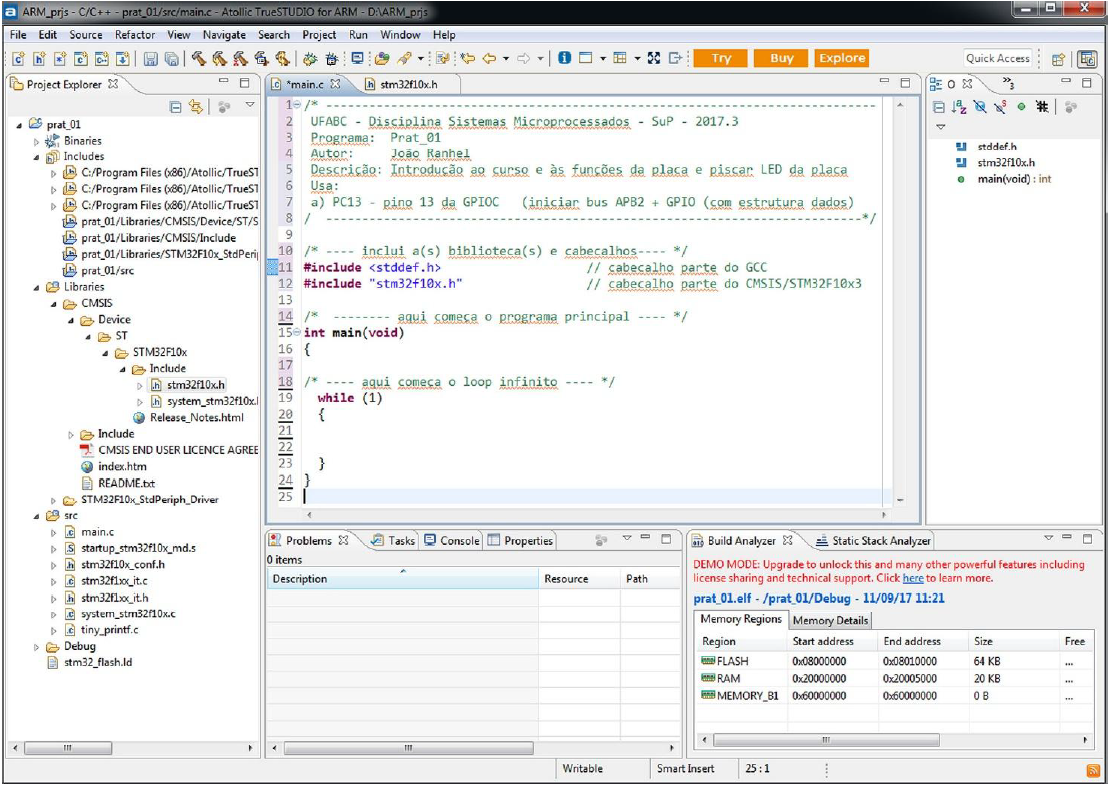
\includegraphics[width=0.8\textwidth]{figures/atollic}
	\caption{Interface Atollic \cite{apostila_microprossados}}
\end{figure}

